%% Author: Daniel Kaplan
%% Subject: Data tables
%% Title: How Many Variables?

Here is part of a spreadsheet on family structure in the US military.  In addition to the table shown in the figure which gives the total across the Department of Defense, there are four additional tabs  for the different branches of the military: Air Force, Marine Corps, Navy, and Army.

\bigskip

\centerline{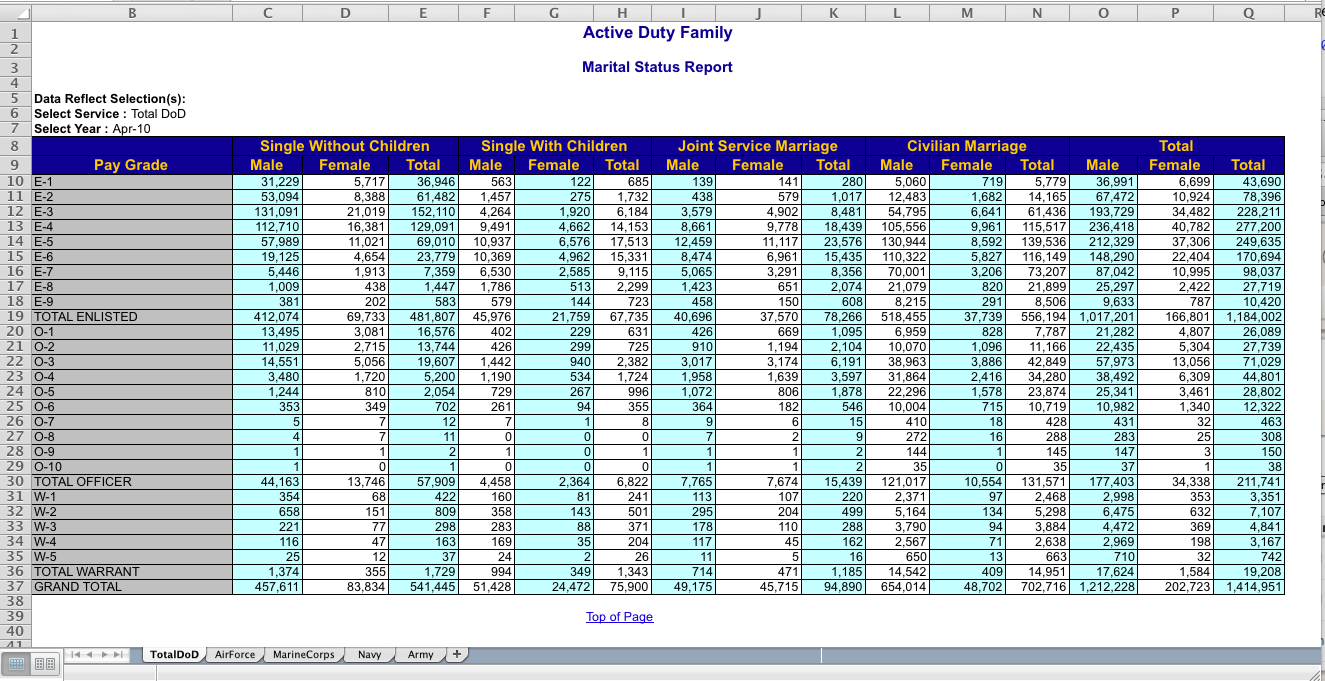
\includegraphics[width=7.5in]{active-duty.png}}

\bigskip

Imagine the data on which the figure is based has an individual person as the unit of analysis.
\begin{enumerate}
\item How many variables are there? 
\item What are the levels for each variable you identified?
\item Which cells in the table (list the row or column number/letter) correspond to tabulations or calculations rather than basic data on the unit of analysis.
\item  Create a short table on Google Docs with just three or four of the cases from different cells in the spreadsheet. Make it publicly available and hand it in.  (Each person in the group should do this.)
\end{enumerate} 
 